\chapter{Material and Methods} \label{methods}
    This chapter describes the steps taken in this thesis to answer the research question:
        \begin{quote}
        "\textit{\textbf{As lightweight vessels may not have the capacity to carry all the six echo sounders the \gls{imr} usually deploys on the Norwegian sandeel surveys, which ones should be prioritized when classifying sandeel in multi-frequency acoustic data?}"}
        \end{quote}
    
    The thesis follows the work of \citeauthor{brautaset2020acoustic}\cite{brautaset2020acoustic}, which was outlined in section \ref{unet_paper_acoustic} and will be referenced throughout this chapter. In summary, this chapter will first look at the data itself and the tools and methods applied to prepare it for the training of machine learning models, with a following description of the experiment. The experiment focuses on training individual models with different subsets of frequencies and measuring the performance of each.
    
    
    % 2019 - 78.76554305432501m
    %2018
    
    
    \section{The Data}
        The data used in this thesis stem from the annual Norwegian acoustic trawl surveys from 2018 and 2019 using the Simrad EK60 echosounder, where 2018 was the same year used by \citet{brautaset2020acoustic}. The data from each year consisted of a collection of \textit{.raw} files. The \textit{.raw} files are the uncompressed raw output from the echo sounder, and stored the backscatter as \gls{sv} values in echograms for six frequencies \textit{18kHz}, \textit{38kHz}, \textit{70kHz}, \textit{120kHz}, \textit{200kHz}, and \textit{333kHz}. Two frequencies (\textit{70kHz} \textit{and} \textit{333kHz}) more than used by \citet{brautaset2020acoustic} . The settings on the echosounder resulted in the size of each pixel representing 1 second horizontally and 19.2 centimeters vertically\cite{choi2021semi} (Visualized in figure \ref{Module_outputs_illustration_fig}). The height and width of the echo sounder data were dependent on the depth measured and the total navigation time of the survey, and the two years used as data in this thesis contained 688 hours of data from 2018 and 1107 hours from 2019.
        %The data originates from the annual Norwegian acoustic trawl surveys using the Simrad EK60 system to measure sandeel abundance and was split into yearly trawl missions. The echo sounder data was provided as \textit{.raw} files, where the backscatter was stored as \gls{sv} values in echograms for six frequencies \textit{18kHz}, \textit{38kHz}, \textit{70kHz}, \textit{120kHz}, \textit{200kHz}, and \textit{333kHz}. By using modules created by 
        
        
        
        %The \textit{.raw} file is the uncompressed raw output from the echo sounder.  The \textit{.work} files are the annotations of the \textit{.raw} files made by operators using the \gls{lsss} system. Backscatter was stored as \gls{sv} values in echograms for six frequencies \textit{18kHz}, \textit{38kHz}, \textit{70kHz}, \textit{120kHz}, \textit{200kHz}, and \textit{333kHz}. The settings on the echosounder resulted in the size of each pixel representing 1 second horizontally and 19.2 centimeters vertically\cite{choi2021semi}.
        
        \section{The CRIMAC-Pipeline Modules}\label{CRIMAC-pipeline}
        Based on the work performed by \citeauthor{brautaset2020acoustic}\cite{brautaset2020acoustic}, a pipeline for classifying the acoustic backscatter was created under \gls{imr}s project \gls{crimac}\cite{crimac_pipeline} and could process the .raw data into a format able to be used by Python. The pipeline could be run as one whole module to get the predictions from the .raw data directly, or submodules of the pipeline (\textit{illustrated in figure \ref{Module_overview_fig}}) could be accessed and run separately. Most of the outputs from modules in the pipeline are of the \textit{.zarr} format. This format stems from the Python Zarr package, which facilitates NumPy array loading and operations through \textit{xarray} on data that is too large to be loaded completely in computer memory (\textit{All tools used are described in appendix \ref{appendix:tools used}}). This section will describe the function of each submodule, hereby called \textit{module}, used in this thesis:
   

        %\subsection{CRIMAC-Pipeline Modules} 
        
                              \begin{figure}[H]
                \centering
                \includesvg[inkscapelatex=false,width=0.9\textwidth,keepaspectratio]{figures/module_overveiw.svg}
                \caption[Module overview]{Module overview and output flowchart. Black represents modules, and other colors represents input/output. The modules' and input/outputs' colors will stay the same for later illustrations.}
              	\medskip 
                \label{Module_overview_fig}
            \end{figure} 
            \begin{description}
            
              \item[$\bullet$ CRIMAC/Preprocessor:] Used to process the \textit{.raw} files to the \textit{.zarr} format, and re-grids all frequency channels to a common range if not equal. The output is a \gls{sv} dataset represented as a single multidimensional array of size $frequency \times ping \times range$ (\textit{One echogram per frequency}). The output \gls{sv} file is illustrated in figure \ref{Module_outputs_illustration_fig}.%The .parquet file acts as bitmaps for each class, but the current version of this module was incompatible with .zarr, and could not produce this file. The solution to this problem is described in section \ref{Pseudo label}. The output \gls{sv} file is illustrated in figure \ref{Module_outputs_illustration_fig}:
                %As the ping rate was set to 1Hz\cite{choi2021semi}, with a pulse duration of 1.024 milliseconds, the length of each pixel is 1 second horizontally and 19.2 centimeters vertically.
                
              \item[$\bullet$ Pretrained CRIMAC/U-Net:] Using a pretrained U-Net model, it produces a segmentation map of pixel-based probabilities with spatial size $class \times ping \times range$. Output classes were \textit{sandeel}, \textit{other}, and \textit{background}. The output predictions is illustrated in figure \ref{Module_outputs_illustration_fig}.
              
              % The \textit{ignore} class is excluded. By changing the settings, we have the option to train a new U-Net model with the same scheme setup in \citeauthor{brautaset2020acoustic}, but it was incompatible with the \textit{.zarr} format and could not be used.
              
              \item[$\bullet$ CRIMAC/Bottom detection:] Identifies the bottom and generates a binary pixel-based map stored as \textit{.zarr}. This is a 2-dimensional array of size $ping \times range$. The output is shown in figure \ref{Module_outputs_illustration_fig}.

            \end{description}
        

        
        \begin{figure}[H]
            \centering
            \includesvg[inkscapelatex=false,width=1\textwidth,keepaspectratio]{figures/output_illustration.svg}
            \caption[Module outputs illustration]{Illustrations of the output from the different modules with one enlarged example from each output. This example is a $500\times500$ crop, while the real data contained millions of pings. The \textit{200kHz} has been transformed to the decibel scale to make the data observable. The color scale is set to be purple at 0 and yellow at 1. White denotes missing values.}
          	\medskip 
            \label{Module_outputs_illustration_fig}
        \end{figure}

    \section{Pseudo Labels} \label{Pseudo label}
         %\citet{brautaset2020acoustic} 
        The operator annotations were unavailable during this work, and so the pretrained CRIMAC/U-Net model was treated as a teacher model, from now called \textit{baseline model}, and it's output as annotations. A hard threshold of 0.8 was applied to the baseline model’s output predictions, and all values below were set to 0, and above to 1, resulting in a hard mask for each class, hereby called the \textit{pseudo labels} (visualized in figure \ref{Pseudo label}). This threshold was applied to only include the most certain predictions of the pretrained CRIMAC/U-Net. As this threshold was applied to all classes, there were instances where a pixel was not assigned to a class.
        
        %The operator annotations of the acoustic data were unavailable during this work, and the solution was to create \textit{pseudo labels} using the aforementioned pretrained CRIMAC/U-Net (section \ref{CRIMAC-pipeline}) module.
        % The operator annotations of the acoustic data were unavailable during this work, and the solution was to create \textit{pseudo labels} using the aforementioned pretrained CRIMAC/U-Net (section \ref{CRIMAC-pipeline}) module. A hard threshold of 0.8 was applied to the output predictions, and all values below were set to 0, and above to 1, resulting in a hard mask for each class. This threshold was applied to only include the most certain predictions of the pretrained CRIMAC/U-Net. As this threshold was applied to all classes, there were some instances where no class was assigned to some pixels. Below is an example pseudo label:
        
        %These labels will contain some noise, as the model they originate from was not perfect. In the next section, I will explain how I handled this. Due to the weighted cross-entropy loss used during training of the model seen in section \ref{unet_paper_acoustic} the background class were usually very noisy, as this class was lowly weighted. This low weight caused the model to care less about classifying the background correctly, and the two samples in figure \ref{data sample fig} illustrates this. As I was to use the same weighting, this did not pose a large problem but explains noise in later illustrations of the background class, and therefore mentioned.

        \begin{figure}[H]
        \centering
        %\subfloat[Low noise background label.]{
        	\label{subfig:correct}
        	\includesvg[inkscapelatex=false,width=1\textwidth,keepaspectratio]{figures/data_sample.svg}
        	%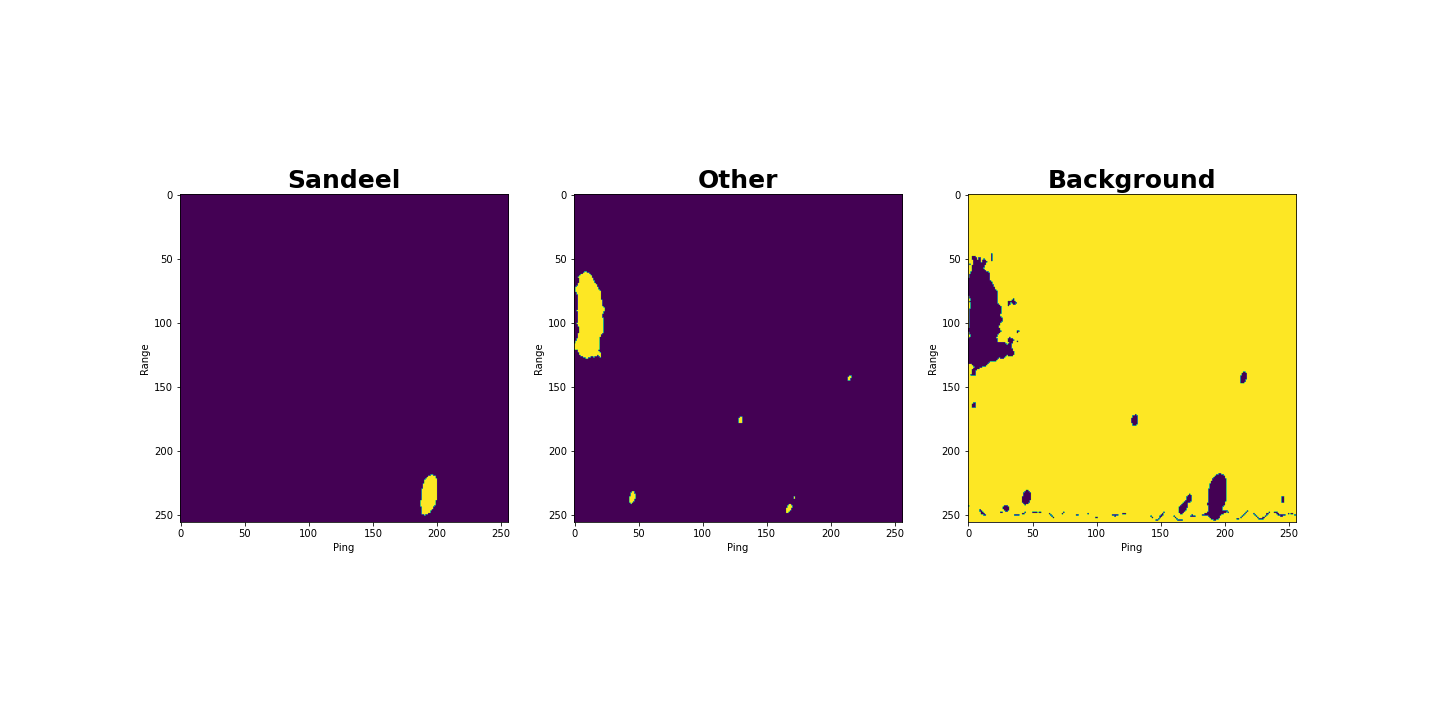
\includegraphics[width=1\textwidth]{figures/data_sample.png} } 
        
        %\subfloat[High noise background label.]{
        	%\label{subfig:notwhitelight}
        	%\includesvg[inkscapelatex=false,width=0.9\textwidth,keepaspectratio]{figures/data_sample_noisy.svg}}
        
        
        \caption[Pseudo label]{An example pseudo label displaying the hard mask of all three classes present in a 256×256 crop: \textit{Sandeel}, \textit{Other}, and \textit{Background}.} %The upper (a) without much noise in the background and the lower (b) containing severe noise.}
        \label{data sample fig}
        
        \end{figure}


        
    \section{Data Preparation}
        This section explains the process of preparing the dataset, which was built to enable a sampling scheme during training equal to the one developed by \citeauthor{brautaset2020acoustic}\cite{brautaset2020acoustic}. The data preparation consists of creating samples with corresponding pseudo labels from the input \gls{sv} data and storing the samples in a folder structure dependent on the sample's features.
        
        The entire process is illustrated in figure \ref{data_generation_flowchart_fig} and starts with utilizing the \gls{crimac} preprocessor module as described in \ref{CRIMAC-pipeline}. This takes in the entire \textit{.raw} dataset and outputs the \gls{sv} data in the \textit{.zarr} format. The \gls{sv} dataset was then sent to both the pretrained U-Net and bottom detection modules from the \gls{crimac} pipeline. The pretrained U-Net outputs pseudo labels, and the bottom detection outputs a mask of the seafloor as arrays equal in spatial size to the \gls{sv} data array.
         %\clearpage
        \begin{figure}[H]
            \centering
            \includesvg[inkscapelatex=false,width=0.75\textwidth,keepaspectratio]{figures/flow_data_gen.svg}
            %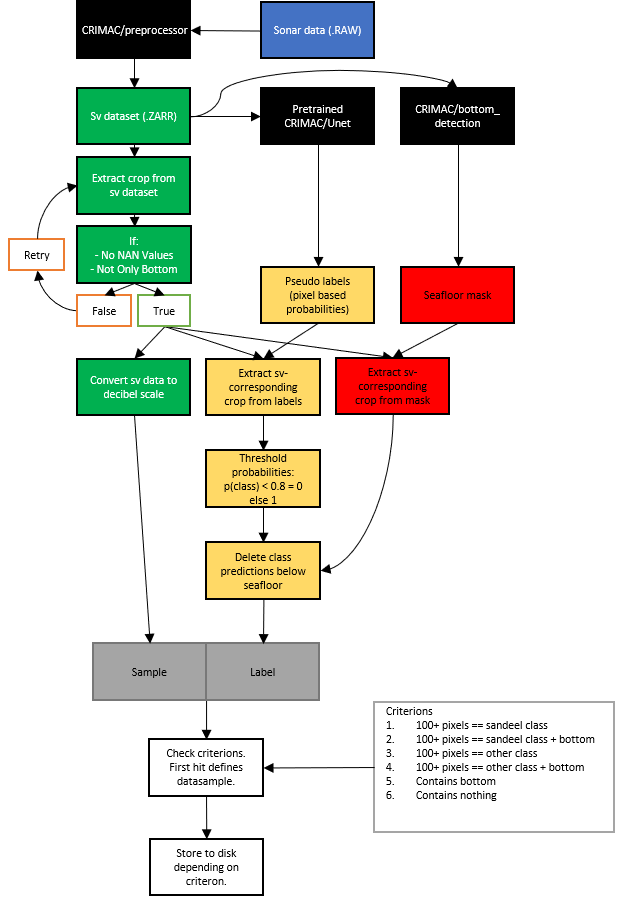
\includegraphics[scale=0.75]{figures/flow_data_gen.png}
            \caption[Data preparation process]{An overview of the data preparation process. CRIMAC pipeline modules (black), data.raw (blue), \gls{sv} data.zarr (green), pseudo labels.zarr (yellow), bottom.zarr (red), the finished file containing two tensors (gray), storing the file with Python pickle (white).}
          	\medskip 
            \label{data_generation_flowchart_fig}
        \end{figure}
        The generated \gls{sv} dataset was then split into non-overlapping crops of size 256x256, ignoring crops of mismatching size at the edges of the array. Each crop was checked for any missing values or the crop being located entirely below the seafloor and then ignored if any of them were true. As visualized in figure \ref{data_bottom_nans_fig} there were instances of discontinuity in both the time series of pings and range. This caused portions of the \gls{sv} dataset to be filled with missing values, hence motivating the previous check as sampling crops at complete random could cause errors.
                \begin{figure}[H]
            \centering
            %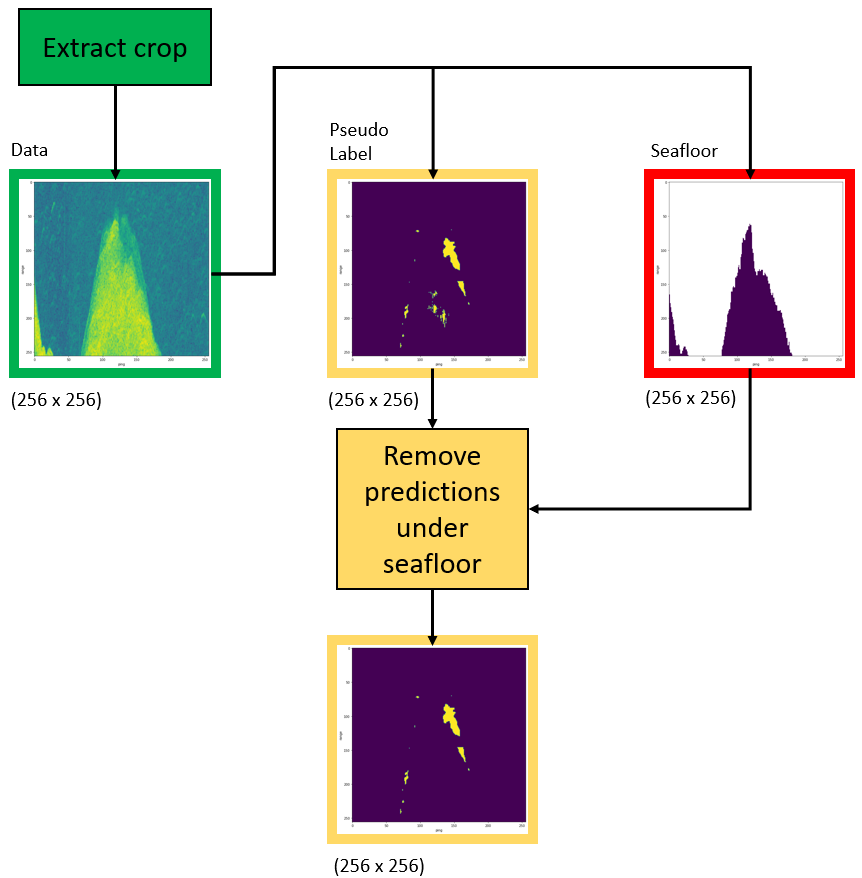
\includegraphics[scale=0.5]{figures/crop_extract_illustration.png}
            \includesvg[inkscapelatex=false,width=0.9\textwidth,keepaspectratio]{figures/data_errors_nans.svg}
            \caption[Missing values and bottom]{Example crop from the 18kHz \gls{sv} data (decibel scale). It illustrates two clear sections of data where the depth (range) is changed, and the gap is filled with missing values (white). The bottom can be observed by the strong line of \gls{sv} values, and there are multiple bottom echoes in certain parts of the crop.}
          	\medskip 
            \label{data_bottom_nans_fig}
        \end{figure}
        %This was because missing values can be detrimental to the training process, and crops below the seafloor were excluded as done by \citeauthor{brautaset2020acoustic}\cite{brautaset2020acoustic}. An illustration of the missing data is illustrated in figure \ref{data_bottom_nans_fig}. 
        
        Using the vertical and horizontal coordinates for all the \gls{sv} data crops, a corresponding crop from both the seafloor mask and the pseudo labels was extracted. The two new crops were then used together to remove predictions that appeared under the bottom, thus cleaning and preprocessing the pseudo labels. The steps explained in this paragraph are also visualized in figure \ref{crop_extract_fig}.

        
        \begin{figure}[H]
            \centering
            %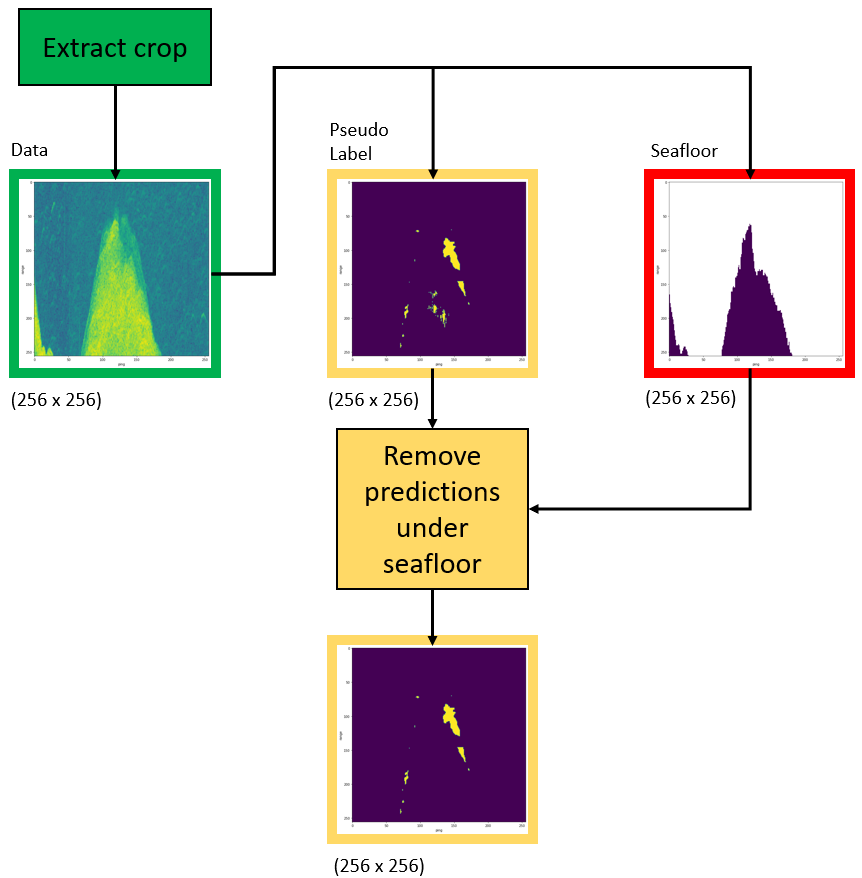
\includegraphics[scale=0.5]{figures/crop_extract_illustration.png}
            \includesvg[inkscapelatex=false,width=0.7\textwidth,keepaspectratio]{figures/crop_extract_illustration.svg}
            \caption[Data, label and bottom crop extraction and interaction]{Example of how the data, pseudo labels, and bottom crops look during data generation. For the pseudo label, purple is values of 0 and yellow values of 1. In the pseudo labels, we can see that some predictions under the seafloor are removed.  Size is shown in the lower-left corner to clarify that it is a crop of the same size and from the same location but from different arrays.}.
          	\medskip 
            \label{crop_extract_fig}
        \end{figure}
        
        After the crop containing the \gls{sv} data and cleaned pseudo labels were generated, they were both converted to tensors and stored as a single file using Python pickle. The storage folder of the file depend on a set of criteria, which are illustrated in figure \ref{data_hierarchy_fig}. The criteria were checked from top to bottom, and the first triggered set the destination folder, creating a folder structure visualized in figure \ref{data_hierarchy_fig}. This also blocked the same crop from appearing in several folders, potentially causing data leakage between datasets.
        \begin{figure}[H]
            \centering
            %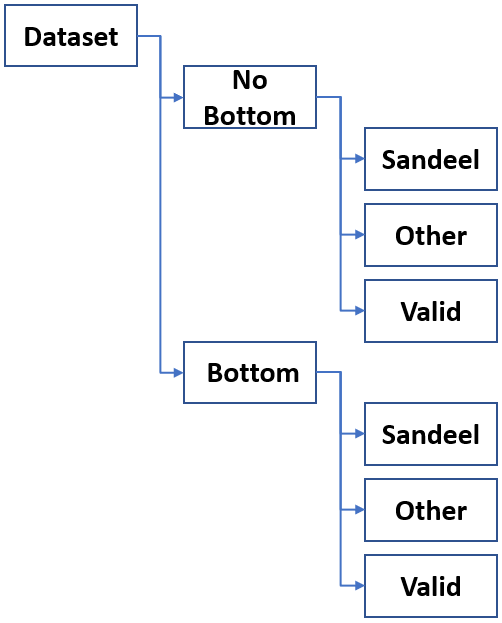
\includegraphics[scale=0.5]{figures/data_hierarki.png}
            \subfloat[The list of criteria.]{
            \includesvg[inkscapelatex=false,width=0.5\textwidth,keepaspectratio]{figures/criteria.svg}}
            
            \subfloat[The folder structure.]{
            \includesvg[inkscapelatex=false,width=0.5\textwidth,keepaspectratio]{figures/folder_structure.svg}}
            


            \caption[Criteria and folder structure]{An overview of the criteria and folder structure. The structure consists of two main branches, one with the bottom present and one without the bottom present.}
            
            
          	\medskip 
            \label{data_hierarchy_fig}
        \end{figure}
        The folder structure and criteria were based on the data classes made by \citeauthor{brautaset2020acoustic}\cite{brautaset2020acoustic}. One significant difference was that they used the actual operator annotations to detect instances of classes in a crop, while we only have the pseudo labels. Since these pseudo labels could contain misclassifications made by the pretrained model, a class abundance measurement was performed. When evaluating the crops against the criteria, if 100 or more pixels in a crop contained either \textit{sandeel} or \textit{other}, the class was set to be present in the crop. This removed crops with low class abundance and where the pretrained model had potentially misclassified single or few pixels. If there were not enough pixels of either class, the crop was set to contain \textit{background} only. The crop from the \gls{sv} data was checked against its corresponding crop from the bottom detector output, splitting the data into folders with or without the bottom present.
        %100 was chosen after trying different criteria and evaluating the number of crops stored in each folder.
                
        %\clearpage


        The years 2018 and 2019 were processed in the way mentioned above individually, and the final data distribution can be seen in respectively table \ref{data_distribution_2018_table} and \ref{data_distribution_2019_table}.



\begin{longtable}{lllllllll}
\caption[2018 data distribution]{Data distribution for the 2018 dataset.}
\\ \cline{1-4}
\multicolumn{2}{|l|}{\textbf{2018 dataset}} & \multicolumn{1}{l|}{Occurrences} & \multicolumn{1}{l|}{\% of dataset} &  &  &  &  &  \\ \cline{1-4}
\endfirsthead
%
\endhead
%
                     & Sandeel              & 1410                             & 7.3\%                              &  &  &  &  &  \\
No bottom            & Other                & 184                              & 0.95\%                             &  &  &  &  &  \\
                     & Background           & 6519                             & 33.75\%                            &  &  &  &  &  \\ \cline{1-4}
                     & Sandeel              & 1297                             & 6.71\%                             &  &  &  &  &  \\
Bottom               & Other                & 840                              & 4.35\%                             &  &  &  &  &  \\
                     & Background           & 9067                             & 46.94\%                            &  &  &  &  &  \\ \cline{1-4}
\multicolumn{2}{l}{\textbf{Total:}}         & 19317                            & 100\%                              &  &  &  &  &  \\ \cline{1-4}
                     &                      &                                  &                                    &  &  &  &  &  \\
                     &                      &                                  &                                    &  &  &  &  & 
\\ \label{data_distribution_2018_table}
\end{longtable}

% Please add the following required packages to your document preamble:
% \usepackage{longtable}
% Note: It may be necessary to compile the document several times to get a multi-page table to line up properly
\begin{longtable}{lllllllll}
\caption[2019 data distribution]{Data distribution for the 2019 dataset.}
\\ \cline{1-4}
\multicolumn{2}{|l|}{\textbf{2019 dataset}} & \multicolumn{1}{l|}{Occurrences} & \multicolumn{1}{l|}{\% of dataset} &  &  &  &  &  \\ \cline{1-4}
\endfirsthead
%
\endhead
%
                     & Sandeel              & 1308                             & 4.38\%                             &  &  &  &  &  \\
No bottom            & Other                & 1074                             & 3.60\%                             &  &  &  &  &  \\
                     & Background           & 10291                            & 34.45\%                            &  &  &  &  &  \\ \cline{1-4}
                     & Sandeel              & 1652                             & 5.53\%                             &  &  &  &  &  \\
Bottom               & Other                & 2815                             & 9.42\%                             &  &  &  &  &  \\
                     & Background           & 12733                            & 42.62\%                            &  &  &  &  &  \\ \cline{1-4}
\multicolumn{2}{l}{\textbf{Total:}}         & 29873                            & 100\%                              &  &  &  &  &  \\ \cline{1-4}
                     &                      &                                  &                                    &  &  &  &  &  \\
                     &                      &                                  &                                    &  &  &  &  & 
\\ \label{data_distribution_2019_table}
\end{longtable}  

        From the tables above, we observe that, as in \citeauthor{brautaset2020acoustic}\cite{brautaset2020acoustic}, most of the data will contain no fish, here represented as \textit{background}.

\clearpage
\section{Experiment} \label{Experiment}
    This section describes how the experiments were performed and how performance was measured, first by describing the settings, then the experiment itself in detail.
    
    \subsection{Experiment Settings} \label{Experiment settings}
        The experiment uses the same U-Net architecture as described in section \ref{unet__brautset_fig} with the alteration developed by \citeauthor{brautaset2020acoustic}\cite{brautaset2020acoustic}. The change to the architecture in this work was to adjust the number of frequency channels in the input layer. This ranged from one to six, depending on the number of frequencies in a subset. All machine learning was implemented using the Python library PyTorch\cite{NEURIPS2019_9015}. %(described in appendix \ref{Pytorch}).
        
        Data loaded to the model started with first selecting a folder from the folder structure, with a set probability for each. Then a sample and a label was extracted at random from this folder, with all samples in each folder being allocated to either training, validation, or test datasets. This imitates the sampling strategy from \citeauthor{brautaset2020acoustic}\cite{brautaset2020acoustic}, and the probabilities originate from this work.
        
        %\clearpage
        \begin{longtable}{lcl}
            \caption[Data loading scheme]{The sample classes correspond to the folder structure described in figure \ref{data_hierarchy_fig}. Each is given a probability of being the target folder for sample extraction.}
            \\ \hline
             \multicolumn{1}{|l|}{\textbf{Sample class}} &  \multicolumn{1}{l|}{\textbf{Probability}} &  \multicolumn{1}{l|}{\textbf{Details}}                                                         \\ \hline
            \endfirsthead
            %
            \endhead
            
            %
            Sandeel                                     & 5/26                                      & Random crop containing the sandeel class                                                      \\ \hline
            Other                                       & 5/26                                      & Random crop containing the other class                                                        \\ \hline
            Background                                       & 1/26                                      & Random crop containing no fish                                                                \\ \hline
            Sandeel + bottom                          & 5/26                                      & \begin{tabular}[c]{@{}l@{}}Random crop containing the sandeel class\\ and bottom\end{tabular} \\ \hline
            Other + bottom                             & 5/26                                      & \begin{tabular}[c]{@{}l@{}}Random crop containing the other class\\ and bottom\end{tabular}   \\ \hline
            Background + bottom                        & 5/26                                      & \begin{tabular}[c]{@{}l@{}}Random crop containing no fish\\ and bottom\end{tabular}           \\ \hline
            \label{Data_loading_scheme_table}
        \end{longtable}

        The data-augmentations performed were flipping along the vertical axis, and a multiplication applied to values in 5\% of pixels in an input \gls{sv} crop to act as noise. An echogram’s orientation of the surface and bottom can never individually be changed during training, so only vertical flipping is justified in acoustic data. The intention behind the multiplication was to simulate real-life noise and consisted of multiplying the values with a random number in either the range [0,1] or [1, 10], with a 50\% chance of each.  As samples from the training data were provided to the model, each data augmentation method had a 50\% chance of occurring. Then the \gls{sv} crop was transformed to the decibel scale by applying $10\log{(pixel)}$ to all pixels for all frequencies in the \gls{sv} crop, with cutoff values at minimum -75dB and maximum 0dB. All augmentations and transformations were based on \citeauthor{brautaset2020acoustic}\cite{brautaset2020acoustic}. 
        
        
        
        %\clearpage
        \begin{longtable}{lll}

            \caption[Data augmentation summary]{Description of each data augmentation performed.}
            \\\hline
            \multicolumn{2}{|l|}{\textbf{Data augmentation}} & \multicolumn{1}{l|}{\textbf{Details}} \\ \hline
            \endfirsthead
            %
            \endhead
            %
            \textit{Add noise to 5\% of pixels.}      &       & 50\% of occurring upon loading sample \\ \hline
            \textit{Flip along the vertical axis}        &       & 50\% of occurring upon loading sample \\ \hline

            \label{data_augmentation_table}
        \end{longtable}
        
        The hyperparameters used during training are summarized in table \ref{hyperparameter_table} and equal those used by \citeauthor{brautaset2020acoustic}\cite{brautaset2020acoustic}.

        \begin{longtable}{lll}
            
            \caption[Experiment hyperparameters]{Settings for all hyperparameters used during the training.}\\
            \\ \hline
            \multicolumn{1}{|l|}{\textbf{Hyperparameters}} & \multicolumn{1}{l|}{\textbf{Value/ Category}} & \multicolumn{1}{l|}{\textbf{Details}}                                                 \\ \hline
            \endfirsthead
            %
            \endhead
            %
            \textit{Loss function:}                         & Weighted Cross-entropy                        & \begin{tabular}[c]{@{}l@{}}Background = 1, \\ Other = 25,\\ Sandeel = 30\end{tabular} \\ \hline
            \textit{Optimizer:}                             & Stochastic gradient descent                   &                                                                                       \\ \hline
            \textit{Learning rate:}                         & 0.01                                          & \begin{tabular}[c]{@{}l@{}}Halved every \\ 1000th batch\end{tabular}                  \\ \hline
            \textit{Momentum:}                              & 0.95                                          &                                                                                       \\ \hline
            \textit{Mini-Batch size:}                            & 16                                            &                                                                                       \\ \hline
            \textit{Crop size:}                             & 256×256                                       & \begin{tabular}[c]{@{}l@{}}Include all \\ available frequency channels\end{tabular}             \\ \hline
        \label{hyperparameter_table}
        \end{longtable}

        To evaluate the performance of the models, we utilized the F1 score mentioned in section \ref{f1_score}. We also included the precision and recall, as these provide greater insight into the model's performance.
        
    %\subsection{Experiment: Training on pseudo labels}
    %  This was a preliminary test to establish that training a model on pseudo labels was possible and would achieve acceptable performance. All frequencies would be included, and this would then produce a baseline performance for the later experiments. 
    
    \subsection{Exhaustive Frequency Search}
        \subsubsection{Description}
        %A comprehensive experiment was enacted to find the most impactful frequencies and try to discover hidden synergies between them. 
        This experiment would see all combinations (\textit{subsets}) of all frequencies being evaluated. Each subset of frequencies would instantiate a new U-Net model based on the architecture described in section \ref{Experiment settings}, with input channels equal to the number of frequencies in the subset. The experiment build on ideas from \gls{kd} and train student models (\textit{the model instantiated by a subset}) on the data labeled by the teacher (\textit{baseline model}). The performance of each subset will be estimated by how well it reconstructs the test data labeled by the teacher. The experiment was run \textit{ten} times to get enough results to estimate the mean, reduce variance, and display statistical data for each subset of frequencies. With six frequencies in total, the number of possible frequency subsets for each experiment is 63\footnote{Calculated as combinations without repetitions and without order, using formula $\frac{n!}{k!(n-k)!}$, where \textit{n} is elements to chose from and \textit{k} is how many to choose, both values as integers. Summarize for \textit{k} in range 1..6.}.  During training, only the frequency channels present in the subset would be extracted from the training data and provided to the model. The ten experiments had different random state seeds set to enable different data splits and variable model initialization. The explicit random state also accommodates reproducibility. 
        
        
        
        The dataset for the year 2019 in table \ref{data_distribution_2019_table} contained the most data and was chosen for training. 30\% of the training dataset was assigned as the validation dataset. Meanwhile, the 2018 dataset was selected as the test dataset. The total amount of data given to a model during training was 5,000 batches. A mini-batch size of 16 corresponds to 80,000 samples, which matches the amount of data given to the model by  \citeauthor{brautaset2020acoustic}\cite{brautaset2020acoustic}.
        
        \subsubsection{Monitoring Training}
        Logging of metrics occured at different stages during the training process;
            \begin{itemize}
                \item Every mini-batch: Calculate the exponential moving average of the training loss.
                \item Every mini-batch: Log the exponential moving average of the training and validation loss.
                \item Every 250 mini-batch: Run model on 100 mini-batches from the validation data, plot one sample output and its label, and calculate  exponential moving average loss on each validation minibatch. Furthermore, calculate F1-score on both training and validation data for where the sandeel class is positive, and the other classes are the negative.
            \end{itemize}
            
        The training process was split into 50 epochs to accommodate this logging scheme, with 100 mini-batches in each. This epoch is only related to the logging scheme, not the data itself. Hence, each epoch is not the entire dataset but a part of a sequence of data. This is mentioned to not confuse a reader observing the results. The metrics loss and F1-score indicate convergence, over-/under-fitting problems, and performance. A sanity check was also performed by observing and judging a prediction of the sandeel class against its label.
        
        \subsubsection{Generalization Performance per Subset}
        After the training of a frequency subset, the subset’s model was evaluated on 500 batches from the test dataset but without any noise added through augmentation. From these predictions, the F1-score, precision, and recall were calculated for where sandeel was the positive class and the two other classes were negative, giving an estimate of its generalization performance. Then the next frequency subset started the entire process afresh with training.
        
        With the results from the ten separate experiments, each on all 63 possible combinations, each frequency subset's mean test performance (\textit{generalization performance}) values were estimated. This was then used to show these properties:
        
        
        \begin{itemize}
            \item A summary of the performance achieved by each subset size.
            \item Finding the best performing frequency combinations per subsets size. One max search based on each metric; F1-score, precision, and recall.
            \item To observe the uniqueness of each subset, a plot to illustrate the statistical properties of each will be presented. This will be shown as error bars, the top of the bars is the max F1-score achieved, and the bottoms is the minimum. %This presentation was chosen because we judged that too few tests had been run for a proper standard deviation to be calculated.
            \item The performance trend of each frequency. This meant, for all frequencies, filtering out those subsets it was a part of and sorting these in increasing order. Producing a line plot illustrating what performance scores each particular frequency contributes to and its overall trend.
        \end{itemize}
    


\section{Hardware} \label{hardware}
    Two remote servers named \textit{Janus} and \textit{Birget} were provided by the University of Bergen. Janus was used for data preparation and Birget for conducting the experiments. Hardware spesifications: 
\begin{itemize}
  \item \textbf{Birget}
  \begin{itemize}
    \item CPU: AMD EPYC 7742 64-Core Processor
    \item GPU: 8 x A100-SXM-80GB (\textit{One available for this thesis})
  \end{itemize}
  \item \textbf{Janus}
  \begin{itemize}
    \item CPU: Intel(R) Core(TM) i9-7900X CPU @ 3.30GHz
    \item GPU: 2 x GeForce RTX 2080 Ti (\textit{One partially available for this thesis})
  \end{itemize}
\end{itemize}